\documentclass[tikz, border=10pt]{standalone}
\usepackage{tikz}
\usetikzlibrary{shapes, arrows.meta, positioning, calc, decorations.markings}

\begin{document}
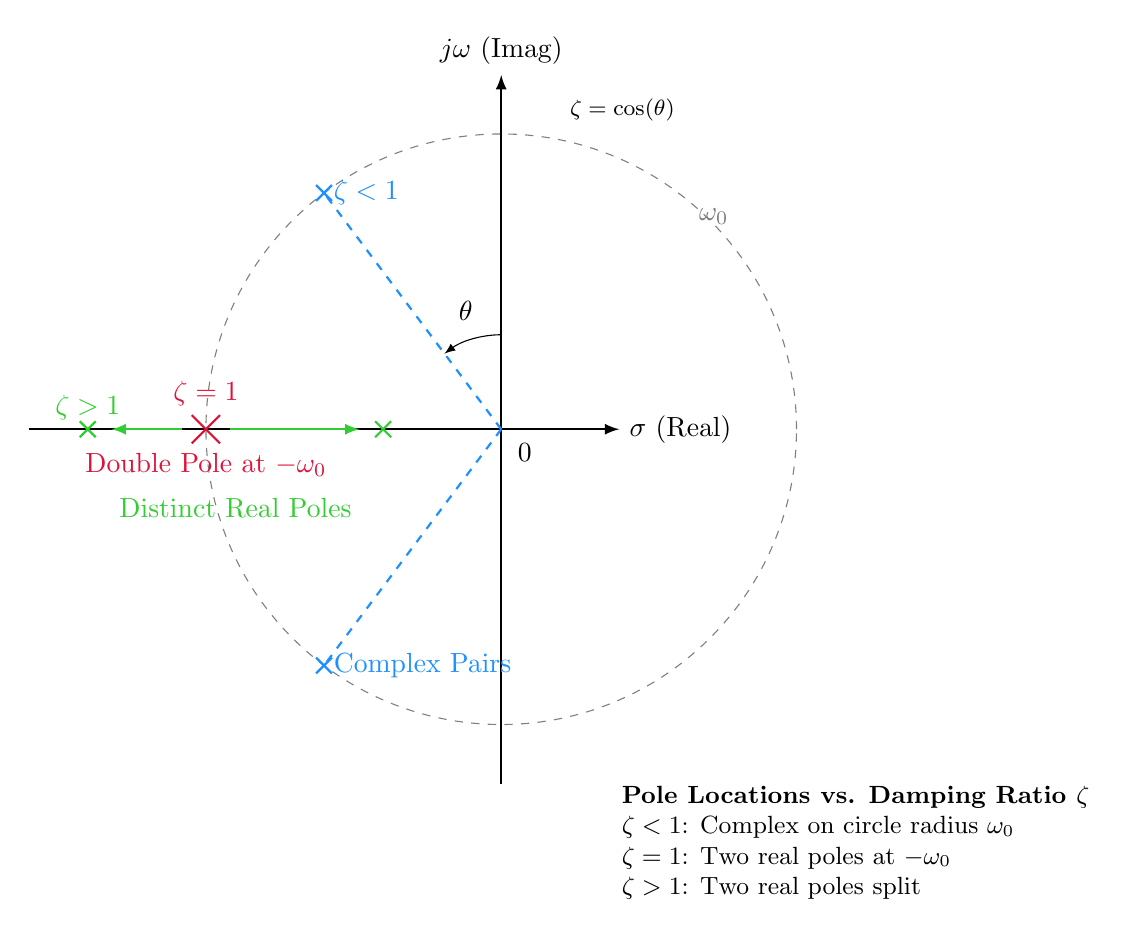
\begin{tikzpicture}[>=latex, scale=1.5]

    % Define colors
    \definecolor{zeta_less}{RGB}{30, 144, 255} % DodgerBlue
    \definecolor{zeta_equal}{RGB}{220, 20, 60} % Crimson
    \definecolor{zeta_more}{RGB}{50, 205, 50}  % LimeGreen

    % Axis
    \draw[->, thick] (-4,0) -- (1,0) node[right] {$\sigma$ (Real)};
    \draw[->, thick] (0,-3) -- (0,3) node[above] {$j\omega$ (Imag)};
    \node at (0.2, -0.2) {0};

    % Circle for zeta < 1
    \draw[dashed, gray] (0,0) circle (2.5);
    \node[gray] at (1.8, 1.8) {$\omega_0$};

    % Locus for zeta < 1 (Complex Conjugates on the circle)
    \coordinate (P1) at (-1.5, 2.0); % Example point
    \coordinate (P2) at (-1.5, -2.0);
    
    \draw[zeta_less, thick, dashed] (0,0) -- (P1);
    \draw[zeta_less, thick, dashed] (0,0) -- (P2);
    
    \node[cross out, draw=zeta_less, thick, scale=1.2, inner sep=2pt] at (P1) {};
    \node[cross out, draw=zeta_less, thick, scale=1.2, inner sep=2pt] at (P2) {};
    
    \node[zeta_less, right] at (P1) {$\zeta < 1$};
    \node[zeta_less, right] at (P2) {Complex Pairs};
    
    % Zeta definition angle
    \draw[->, thin] (0,0.8) arc (90:127:0.8);
    \node at (-0.3, 1.0) {$\theta$};
    \node[right, font=\footnotesize] at (0.5, 2.7) {$\zeta = \cos(\theta)$};

    % Locus for zeta = 1 (Real Double Pole)
    \coordinate (P_crit) at (-2.5, 0);
    \node[cross out, draw=zeta_equal, thick, scale=1.5, inner sep=3pt] at (P_crit) {};
    \node[zeta_equal, above=5pt] at (P_crit) {$\zeta = 1$};
    \node[zeta_equal, below=5pt] at (P_crit) {Double Pole at $-\omega_0$};

    % Locus for zeta > 1 (Real Distinct Poles)
    \coordinate (P_over1) at (-3.5, 0);
    \coordinate (P_over2) at (-1.0, 0); % Just an example separation
    
    % Arrows showing movement for zeta > 1
    \draw[->, zeta_more, thick] (-2.7, 0) -- (-3.3, 0);
    \draw[->, zeta_more, thick] (-2.3, 0) -- (-1.2, 0);

    \node[cross out, draw=zeta_more, thick, scale=1.2, inner sep=2pt] at (P_over1) {};
    \node[cross out, draw=zeta_more, thick, scale=1.2, inner sep=2pt] at (P_over2) {};
    
    \node[zeta_more, above] at (P_over1) {$\zeta > 1$};
    \node[zeta_more, below] at (-2.25, -0.5) {Distinct Real Poles};

    % Annotations
    \node[align=left, font=\small] at (3, -3.5) {
        \textbf{Pole Locations vs. Damping Ratio $\zeta$} \\
        $\zeta < 1$: Complex on circle radius $\omega_0$ \\
        $\zeta = 1$: Two real poles at $-\omega_0$ \\
        $\zeta > 1$: Two real poles split
    };

\end{tikzpicture}
\end{document}
